\cleardoublepageforprint	% In print mode, this will do a \cleardoublepage, otherwise just a \clearpage

\chapter{Example Chapter}
\label{chap:example}

Here is a link to the Research Questions in Section~\ref{sec:example.rq}. There is also this very fine Figure ~\ref{fig:example.c}. I also want to draw your attention to the information in this footnote\footnote{Footnotes are like bicycles -- there is always room for n+1}. Of course we must also consider \citet{leach2018iain} and \citet{martin2021shadow}.

\lipsum[2]

\section{Example Section}
\label{sec:example.examplesec}

\lipsum[2]

\begin{figure}[h!]
	\centering
	\captionsetup{justification=centering}
	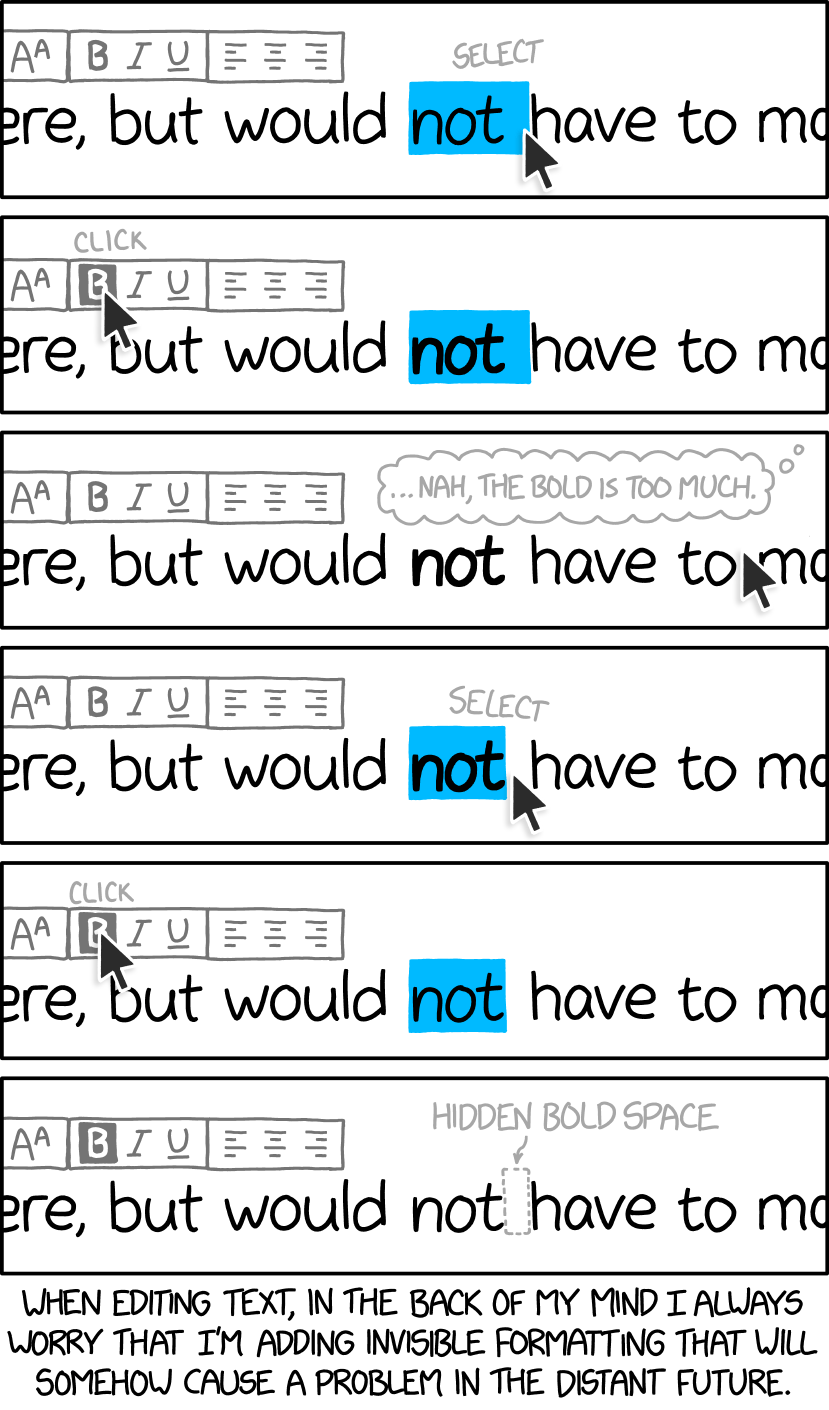
\includegraphics[height=8cm]{images/examples/xkcd_2109_invisible_formatting_2x.png}
	\caption[Example figure A]{Example figure that should probably be removed at some point\protect\footnotemark}
	\label{fig:example.a}
\end{figure}
\footnotetext{Attribution: xkcd 1205 (\url{https://xkcd.com/1205})}

\section{Links}
\label{sec:example.links}

\subsection{DOI}
\label{sec:example.links.doi}


This is an example of a DOI being linked: [\hyperrefDoi{\doiExampleDocument}{hyperdarkerblue}].

On the other hand here we reference a path in a resources bundle:\\
\hyperrefDoiWithPath{\doiExampleRepository}{/some/example/document.txt}

\subsection{Perma}
\label{sec:example.links.perma}

Here is a URL with an associated \texttt{perma.cc} link:\\
\urlWithPerma{https://xkcd.com/327/}{EP49-TCM6}

You could also have that as a footnote\footnoteUrlWithPerma{https://xkcd.com/327/}{EP49-TCM6}.

\vspace{1em}

\clearpage

\section{Research Questions}
\label{sec:example.rq}

We formulated the following research questions and hypotheses.  We will later go on to reflect on these in our final chapter [\ref{sec:example2.rq}].

\subsection{Non-coercive Diplomatic Frameworks}
\label{subsec:example.rq.diplomatic}

\begin{researchquestion}
	\label{rq:diplomatic}
	\RQDiplomatic
\end{researchquestion}

We propose the following hypotheses in relation to this question, in order to frame the research and guide the methodology:

\begin{hypothesis}
	\label{hyp:diplomatic.first}
	\HDiplomaticA
\end{hypothesis}

\begin{hypothesis}
	\label{hyp:diplomatic.second}
	\HDiplomaticB
\end{hypothesis}

\clearpage

\subsection{AI Mediators}
\label{subsec:example.rq.minds}

\begin{researchquestion}
	\label{rq:minds}
	\RQMinds
\end{researchquestion}

This primary research question has the following sub-questions:

\begin{subquestion}
	\label{srq:minds.a}
	\SRQMindsA
\end{subquestion}

\begin{subquestion}
	\label{srq:minds.b}
	\SRQMindsB
\end{subquestion}

We propose the following hypotheses in relation to this question:

\begin{hypothesis}
	\label{hyp:minds.first}
	\HMindsA
\end{hypothesis}

\begin{hypothesis}
	\label{hyp:minds.second}
	\HMindsB
\end{hypothesis}


\clearpage


\section{Another Example}
\label{sec:example.another}

\begin{figure}[h!]
	\centering
	\captionsetup{justification=centering}
	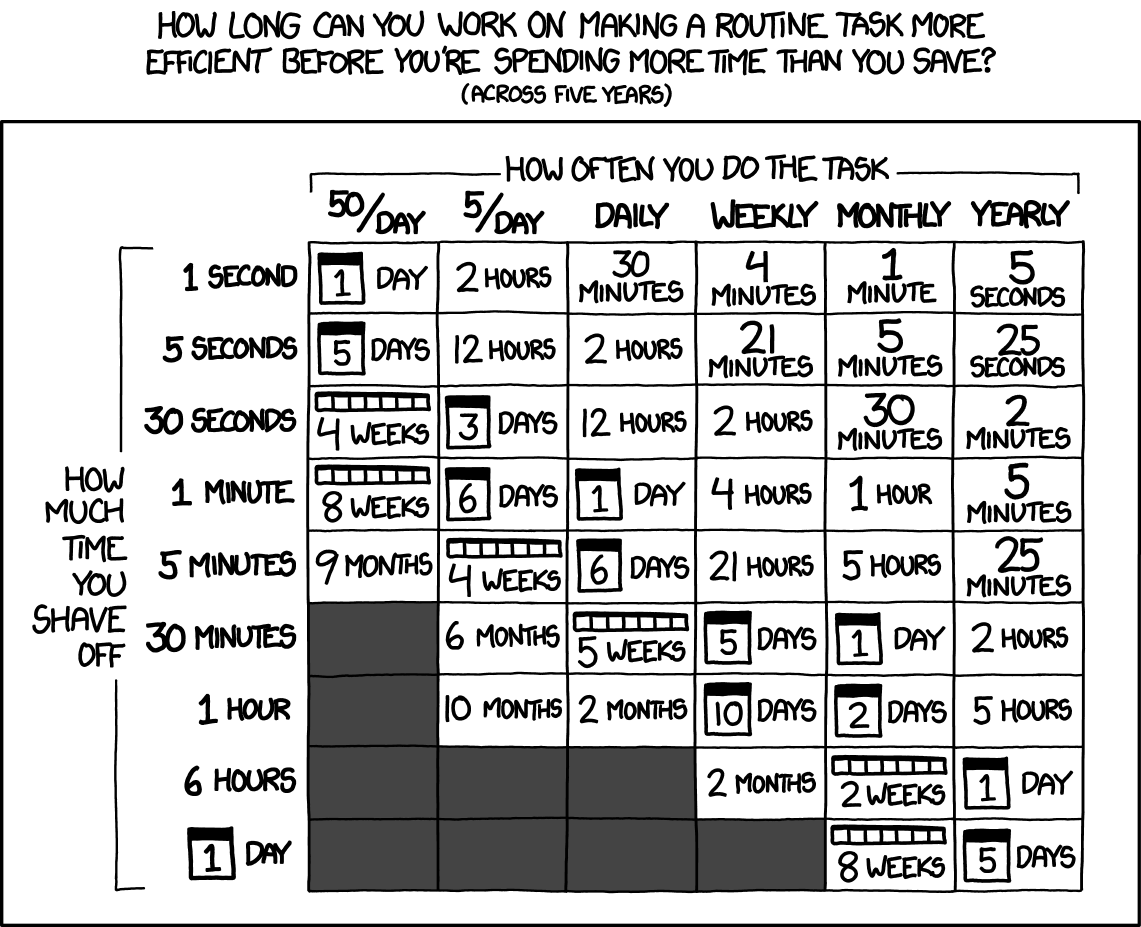
\includegraphics[height=9cm]{images/examples/xkcd_1205_is_it_worth_the_time_2x.png}
	\caption[Example figure B]{I feel this table is relevant to many aspects of PhD work\protect\footnotemark}
	\label{fig:example.b}
\end{figure}
\footnotetext{Attribution: xkcd 2109 (\url{https://xkcd.com/2109})}

\lipsum[4]

\begin{figure}[h!]
	\centering
	\captionsetup{justification=centering}
	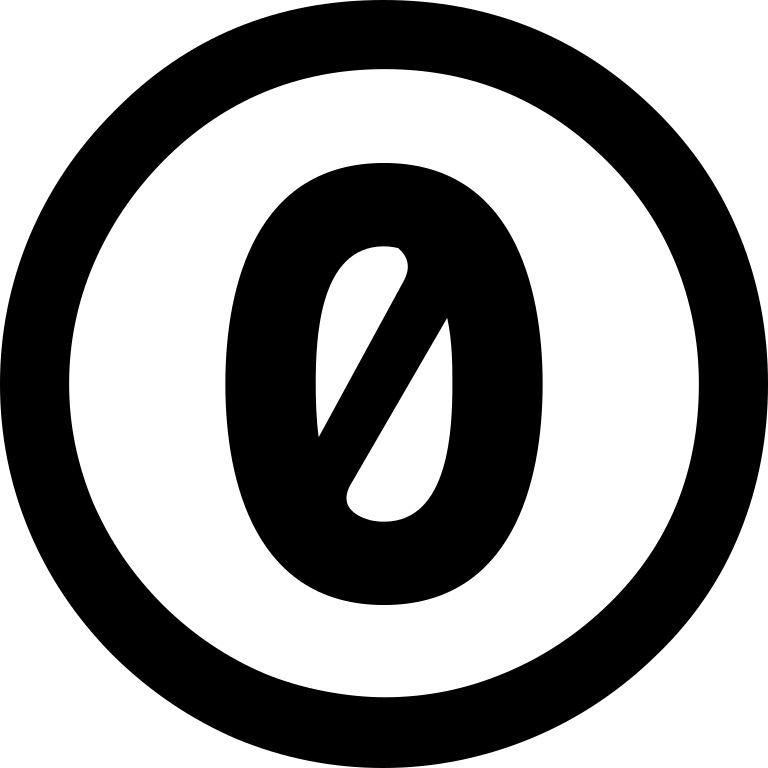
\includegraphics[height=5cm]{images/examples/cc-zero.png}
	\caption{Example figure with no attribution}
	\label{fig:example.c}
\end{figure}


\clearpage

\subsection{Foo}
\label{subsec:example.another_foo}

\begin{table}[h]
	\centering
	\caption{\textit{Some important numbers}}
	\small{
		\renewcommand{\arraystretch}{1.4} 
		{%
			\scalebox{0.86}{
				{\begin{tabular}{|p{5.5cm}|>{\centering\arraybackslash}p{2cm}|p{8cm}|}
						\hline
						\rowcolor[HTML]{EFEFEF} 
						{\color[HTML]{000000} \textbf{Response}} & {\color[HTML]{000000} \textbf{Frequency}} & {\color[HTML]{000000} \textbf{Note}} \\ \hline
						\rowcolor[HTML]{FFFFFF} 
						1 (Strongly disagree) & 1 & Not at all happy \\ \hline
						\rowcolor[HTML]{FFFFFF} 
						2 (Disagree) & 0 & Meh \\ \hline
						\rowcolor[HTML]{33FFFF} 
						3 (Dunno) & 2 & Middle of the road \\ \hline
						\rowcolor[HTML]{FFFFFF} 
						4 (Agree) & 12 & So-so \\ \hline
						\rowcolor[HTML]{FFFFFF} 
						5 (Strongly agree) & 9 & Very happy  \\ \hline
					\end{tabular}%
	}}}}
	\label{tab:example.a}
\end{table}


\begin{theorem}[Pythagorean theorem]
	\label{the:example.pythagorean}
	This is a theorem about right triangles and can be summarised in the next 
	equation: 
	\[ x^2 + y^2 = z^2 \]
\end{theorem}

And a consequence of theorem \ref{the:example.pythagorean} is the statement in the next 
corollary.

\begin{corollary}
	There's no right rectangle whose sides measure 3cm, 4cm, and 6cm.
\end{corollary}

\begin{lemma}
	Given two line segments whose lengths are \(a\) and \(b\) respectively there is a 
	real number \(r\) such that \(b=ra\).
\end{lemma}


\lipsum[7]

\clearpage


Table \ref{tab:example_long_table} is an example of a long table split over multiple pages.

\vspace{10mm}

\begin{small}

\begin{longtable}{|p{3cm}|c|p{4cm}|}
	
	\caption{Example multi-page table} \label{tab:example_long_table} \\
	\hline 

	\textbf{Column 1} & \textbf{Column 2} & \textbf{Column 3} \\ \hline
	\endfirsthead
	
	\multicolumn{3}{c}{{\bfseries \tablename\ \thetable{} -- continued from previous page}} \\
	\hline \textbf{Column 1} & \textbf{Column 2} & \textbf{Column 3} \\ \hline
	
	\endhead
	
	\hline \multicolumn{3}{|r|}{{\footnotesize\textit{Continued on next page}}} \\ \hline
	\endfoot
	
	\hline \hline
	\endlastfoot
	
	\multicolumn{3}{|>{\raggedright\arraybackslash}S{p{10cm}}|}{\footnotesize\textbf{This is a subheading in the table that stretches over all the columns}} \\
	\hline
	
	A & 1 & Foo \\ \hline
	B & 2 & Bar \\ \hline
	C & 3 & Baz\\ \hline
	
	\multicolumn{3}{|>{\raggedright\arraybackslash}S{p{10cm}}|}{\footnotesize\textbf{This is another subheading}} \\
	\hline
	
	D & 1 & Foo \\ \hline
	E & 2 & Bar \\ \hline
	F & 3 & Baz\\ \hline
	
	\multicolumn{3}{|>{\raggedright\arraybackslash}p{10cm}|}{\footnotesize\textbf{And so is this}} \\ \hline

	G & 1 & Foo \\ \hline
	H & 2 & Bar \\ \hline
	I & 3 & Baz\\ \hline

	\multicolumn{3}{|>{\raggedright\arraybackslash}p{10cm}|}{\footnotesize\textbf{And this}} \\ \hline
	
	J & 1 & Foo \\ \hline
	K & 2 & Bar \\ \hline
	L & 3 & Baz\\ \hline

	\multicolumn{3}{|>{\raggedright\arraybackslash}p{10cm}|}{\footnotesize\textbf{Also this}} \\ \hline
	
	M & 1 & Foo \\ \hline
	N & 2 & Bar \\ \hline
	O & 3 & Baz\\ \hline

	\multicolumn{3}{|>{\raggedright\arraybackslash}p{10cm}|}{\footnotesize\textbf{This too}} \\ \hline
	
	P & 1 & Foo \\ \hline
	Q & 2 & Bar \\ \hline
	R & 3 & Baz\\ \hline


	\multicolumn{3}{|>{\raggedright\arraybackslash}p{10cm}|}{\footnotesize\textbf{Once again}} \\ \hline

	S & 1 & Foo \\ \hline
	T & 2 & Bar \\ \hline
	U & 3 & Baz\\ \hline


	\multicolumn{3}{|>{\raggedright\arraybackslash}p{10cm}|}{\footnotesize\textbf{Finally, so this is}} \\ \hline

	V & 1 & Foo \\ \hline
	W & 2 & Bar \\ \hline
	X & 3 & Baz\\ \hline

\end{longtable}

\end{small}

\clearpage


\section{Incuding Files Via Inputs}
\label{sec:example.inputs}


\noindent
\phantomsection
\begin{minipage}[t]{0.15\textwidth}
	\centering
	\textbf{Type 1} \par
	\textit{Category A} \par
	\label{example-1:1.a}
\end{minipage}
\hspace{0.5cm}
\begin{minipage}[t]{0.8\textwidth}
	\textbf{This is the title of the item} \par
	This is some text.  In this case we have defined a couple of footnotes\footnote{Like this one} to show how they are shown when we have minipages formatted like this.  We can also use this type of footnote\footnoteUrlWithPerma{https://xkcd.com/327/}{EP49-TCM6}.
\end{minipage}
\vspace{0.5cm}

\noindent
\phantomsection
\begin{minipage}[t]{0.15\textwidth}
	\centering
	\textbf{Type 1} \par
	\textit{Category B} \par
	\label{example-1:1.b}
\end{minipage}
\hspace{0.5cm}
\begin{minipage}[t]{0.8\textwidth}
	\textbf{This is the title of the item} \par
	\lipsum[4]
\end{minipage}
\vspace{0.5cm}

\noindent
\phantomsection
\begin{minipage}[t]{0.15\textwidth}
	\centering
	\textbf{Type 2} \par
	\textit{Category C} \par
	\label{example-1:2.c}
\end{minipage}
\hspace{0.5cm}
\begin{minipage}[t]{0.8\textwidth}
	\textbf{This is also a title} \par
	\lipsum[5]
\end{minipage}
\vspace{0.5cm}

